% !TEX root = ../main.tex
% §3 Task Definition & Data. Numbers from results/stage4_eda/{eda_summary,eda_split_counts,eda_imbalance,
% eda_crop_loss}.csv; Tier 2 feature size from results/stage6_main/search_log.txt (chosen config).
\section{Task Definition \& Data}
\label{sec:data}

\paragraph{Anomaly definition and unit of detection.}
This is an image anomaly detection task: industrial inspection photographs, where the challenge is
spatial texture, background clutter and very small defects.
The unit of detection is one image of one product.
An image is \emph{normal} if the object meets specification, and \emph{anomalous} if it shows a surface
defect (scratch, burn, colour spot, crack, bubble) or a structural defect (bent, misplaced or missing
part).
Figure~\ref{fig:samples} shows one normal and one anomalous image for four objects.
The defects are small: the median ground-truth mask covers 0.20\% of the image (10th / 90th
percentile: 0.03\% / 1.67\%).

\begin{figure*}[t]
  \centering
  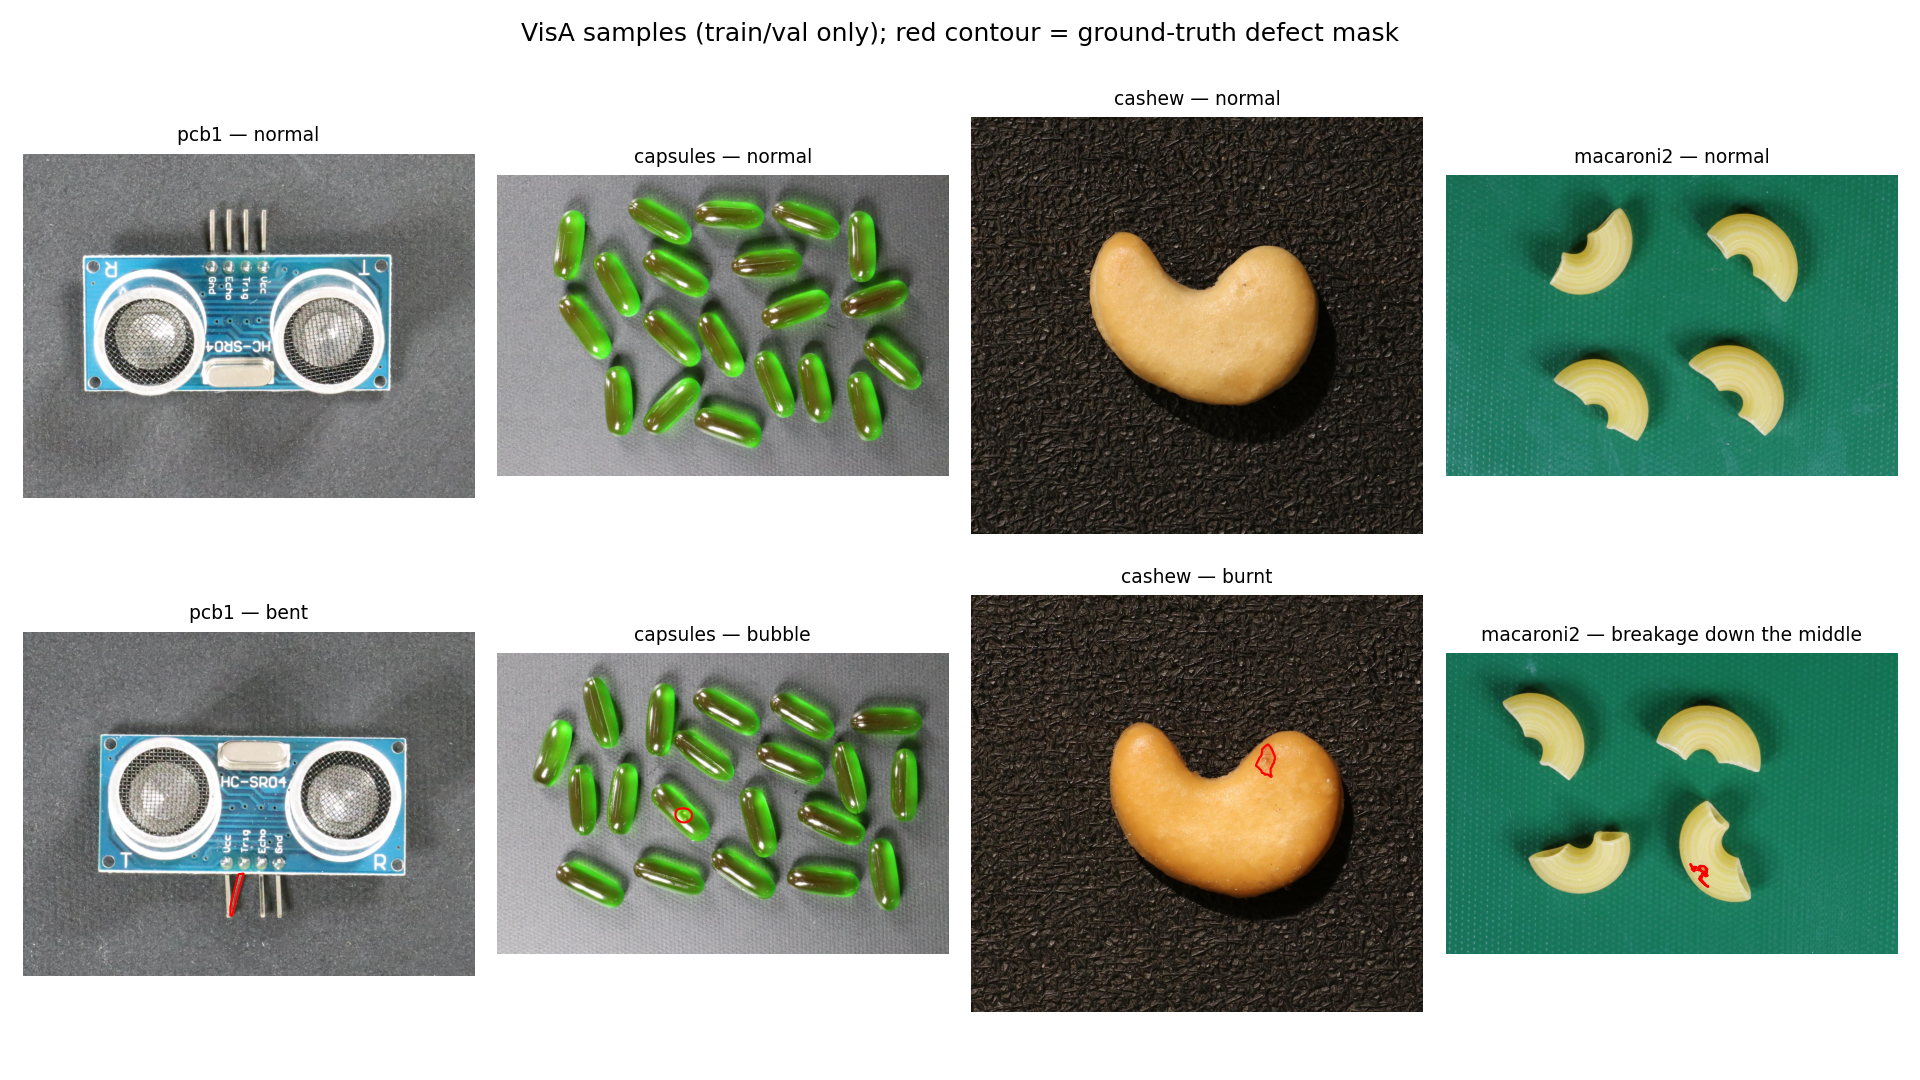
\includegraphics[width=0.8\textwidth]{stage4_eda/fig_samples.png}
  \caption{Normal (top) and anomalous (bottom) VisA images for four of the 12 objects, taken from train and
    validation only. Red contours mark the ground-truth defect masks.}
  \label{fig:samples}
\end{figure*}

\paragraph{Dataset.}
We use VisA \citep{zou2022spot}, released under CC BY 4.0 at
\url{https://github.com/amazon-science/spot-diff}.
It contains $N = 10{,}821$ images, of which 9,621 are normal and 1,200 anomalous.
They cover 12 objects in three groups: complex structure (pcb1--4), multiple instances (candle, capsules,
macaroni1--2) and single instance (cashew, chewing gum, fryum, pipe fryum), with 34 defect types in total.
Raw images are 1,274--1,562\,px wide and 960--1,176\,px high.
Every tier receives a $224 \times 224 \times 3$ input ($D = 150{,}528$).
Tiers~2 and~3 work on pretrained patch features instead of pixels: 3,584 channels per location for
Tier~2 (reduced to 200, \S\ref{sec:method}) and 1,536 for Tier~3.
Table~\ref{tab:data} summarises the data.

\paragraph{Labels and paradigm.}
Image-level labels and pixel masks are provided by the dataset authors; we use the masks only for
analysis, never for training.
Subtle defects may carry label noise, which we cannot quantify.
For capsules every anomaly carries the same defect label (bubble), so the per-type stratification
below reduces to random sampling for that object.
The setting is semi-supervised: every model is fitted on normal images only, and a small set of labelled
anomalies is used only to choose thresholds and hyperparameters.

\paragraph{Split.}
Starting from the official one-class split, we fix one split (seed~0) and share it across all tiers
(Table~\ref{tab:data}).
For each object, 89\% of the official training normals form \emph{train}.
The other 11\% plus 20 anomalies form \emph{val}.
Another 20 anomalies form a \emph{contamination pool}, used only in the training-contamination
ablation.
The official test normals plus the remaining 60 anomalies form \emph{test}.
Anomalies are stratified by defect type, and no image appears in two splits.

\begin{table}[t]
  \centering
  \small
  \begin{tabular}{@{}lrrr@{}}
    \toprule
    Subset & Normal & Anomaly & Anomaly \% \\
    \midrule
    Full dataset       & 9,621 & 1,200 & 11.1 \\
    Train              & 7,705 &     0 &  0.0 \\
    Val                &   954 &   240 & 20.1 \\
    Contamination pool &     0 &   240 & -- \\
    Test               &   962 &   720 & 42.8 \\
    \midrule
    \multicolumn{4}{@{}l}{Objects 12; defect types 34; median defect area 0.20\%} \\
    \multicolumn{4}{@{}l}{Raw size $\approx$1,400\,$\times$\,1,070\,px; input $224 \times 224 \times 3$} \\
    \bottomrule
  \end{tabular}
  \caption{VisA summary and our split (all 12 objects). Train, val and test use 20 / 20 / 60
    anomalies per object; ``raw size'' is the median width $\times$ height.}
  \label{tab:data}
\end{table}

\paragraph{Preprocessing.}
Images are resized directly to $224 \times 224$ and normalised with ImageNet statistics.
We do not use the common resize-256 plus centre-crop-224.
On val masks that crop would remove 4.1\% of defect pixels on average, 10.9\% for capsules and 22.9\% for
macaroni2, where 12.5\% of the defects would be cut out entirely.

\paragraph{Class imbalance.}
The anomaly : normal ratio is 1 : 8.02 over the full dataset (11.1\% anomalies), 1 : 3.98 in val and
1 : 1.34 in test (42.8\%).
Both are far above a realistic production prevalence.
A predict-all-normal rule reaches 57.2\% test accuracy, and would reach 99.0\% at a 1\% prevalence while
catching no defect, so we never report accuracy.
A classifier trained with plain cross-entropy on such data would drift towards the same rule.
We avoid that failure in three ways.
First, all models are fitted on normal images only, so the rare class never enters a loss.
Second, the primary metric is PR-AUC, which, unlike ROC-AUC, depends on the anomaly rate
\citep{davis2006relationship,saito2015precision}.
Third, we convert each operating point to the precision expected at a deployment prevalence $\pi$:
\begin{equation}
  \mathrm{prec}_\pi = \frac{\pi \cdot \mathrm{TPR}}{\pi \cdot \mathrm{TPR} + (1-\pi) \cdot \mathrm{FPR}},
  \label{eq:prec-pi}
\end{equation}
with $\pi \in \{1\%, 5\%\}$.
